\chapter{Experimental setup.} 
\commento{
\begin{itemize}
\item description of MAMI, how the beam is produced, how the electrons are polarized.
\item description of A1.
\item description of beam stabilization, how the monitors measure the beam parameters.
\item Electronics description, DAQ system, VFC monitors.
\item Detectors A and B.
\end{itemize}}

\section{Overview of the experiment.} \label{FirstDescription}

To measure the Beam-Normal single spin asymmetry, a polarized beam of $ \SI{570}{\mega \electronvolt}$ will be sent against a $\SI{10}{\milli \meter}$ width of $^{12}C$ target. The detectors consist of two fused-silica coupled to 3 (detector B) and 8 (detector A) pmts, which collect the Cherenkov light emitted when an electron pass through the fused-silica. 
The detector are placed inside the two spectrometer of the A1 hall, which are not used in this experiment due to the high luminosity of the beam ($ \SI{20}{\micro \ampere}$) that is away from their good point of operation. 
The photomultipliers asymmetry due the change of the electrons spin is the target of the measurement. The pmts signals are collected and digitalized by the \textbf{NINO} board, after a threshold selection, and sent to the A1 control room computer, where the DAQ program collect the data together with all the data coming from the Beam monitors producing Binary files, which are later analyzed by the analysis program, which is significant part of the work done in the framework of the thesis. 
The data collected are divided in \textit{Events} made by 4 \textit{sub-events} in sequence. Each event correspond to a temporal window of $\simeq \SI{80}{\micro \second}$, where each sub-event is $\SI{20}{\micro \second}$ long. Here it's important to clarify that unlike the majority of experiments in high energy physics, an event is made by all the electrons interacting with the detectors during the time interval of the event, and we will refer to this hereafter unless otherwise stated. The division into sub-events reflects the polarization sequence of the beam. The PMTS counts and the beam monitor values are saved for each subevent, along with the time lenght of the event (measured by in clock cycle by the NINO electronic board \ref{NINO}), and other values which are required to process beam monitor data.\\ 

The general structure of the event is the following: 

\begin{figure}[hbtp]
\centering
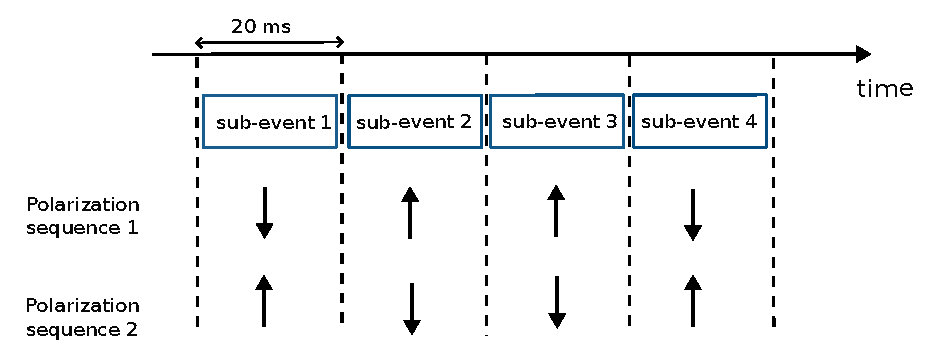
\includegraphics[width = 0.55\textwidth]{ExperimentalSetup/EventStructure.pdf}
\caption{Event structure}
\end{figure}

The two polarity pattern are selected randomly using a De Brujing sequence, (\textbf{spiegare cosa è e come è implementata}). For each event the asymmetry $A_{n}$ is computed, along with 

\newpage
\section{Mami}
\commento{ How Mami produces polarized electron and how the particle are accelerated (the way Mainz Mikroton is working is completely different from the other accelerators, so maybe this section will be too long).}

\subsection{Acceleration stage.}
\commento{explain how electrons are accelerated, and sent to different experiments.} \medskip

\subsection{Polarized Beam.}
\commento{Here a subsection to explain how the polarized electrons are produced. Important to mention the systematic error for the polarization mesurement (in our beam time we couldn't measure with Moller polarimeter, so this discussion is important for future experiment, however it's important to say something about it). Remember to explain how the spin are rotated to the transverse plane, and the $\frac{\lambda}{2}$} \medskip

For the beam-normal single spin asymmetry a vertical polarized beam is necessary. At the MAMI electron accelerator is possible to produce a vertical polarized beam with energy in the range $\SI{180}{\mega \electronvolt} - \SI{855}{\mega \electronvolt}$ \cite{Schlimme_2017}. In this section the procedure to orient the beam vertically is presented, following an explanation of how the degree of polarizarion of the beam is measured. \medskip

The electron source used at MAMI is made by a strained GaAs/GaAsP superlattice photocathode illuminated by circular polarized light. A Pockels cell changes the helicity of the photons impinging on the electrons. The extracted electron has the same helicity of the incoming photon, let's suppose as an example:

\begin{center}
\begin{equation}
\feynmandiagram [scale = 0.8, transform shape][baseline = (g)]{
	a [particle = \(e^{-}\)] -- [fermion] b  -- [fermion] c [particle = \(e^{-}\)],
	b -- [boson] d [particle = \(\gamma\)],};
\hspace{2cm}
(Jz)_{\gamma} = \pm 1 \qquad (Jz)_{e^{-}} = \mp \frac{1}{2} \rightarrow \pm \frac{1}{2}
\end{equation}
\end{center}

With the fast change of the Pockels cell it is possible to alternately revert the sign of the polaritazion. By the insertion of a $\lambda/2$ plate between the laser system and the photochatode the polarization orientation of the electron beam can be reversed for each sub-event, useful later for the estimation of systematic errors. The beam polarization achieved with this source is roughly $80 \% $, for the beam time it was : $0.79 \% $

To switch from longitudinal polarization to transverse polarisation, two devices are used: the \textbf{Wien filter} and a \textbf{double solenoid} located in the injection beam line. 

\begin{figure}[hbtp]
\centering
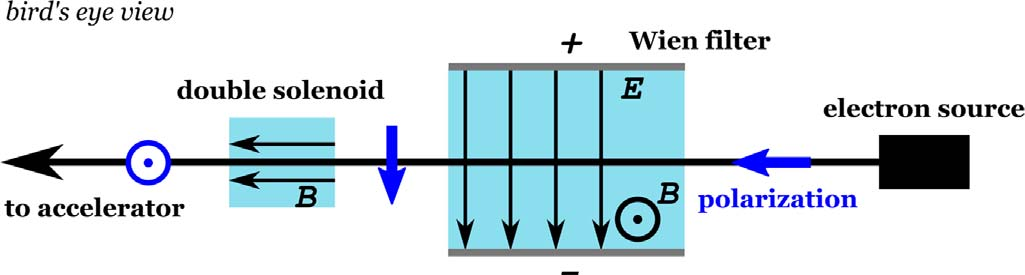
\includegraphics[width = \textwidth]{ExperimentalSetup/injection.png}
\caption{Setup for the trasverse polarization.}
\end{figure}

Following the picture, the longitudinal polarized electron from the source are rotated first in the XY plane, to obtain the trasverse polarization, then with subsequent double solenoid the spins are rotate in the vertival direction. 
After this allignement the electrons go through the accelerator to the experimental hall. The spins then precesses during this time in the magnetic fields of the accelerator's bending magnets, following the BMT equation.
In our experiment, because of the vertical polarization, only the residual horizontal component precedes during the motion. For conventional experiment the polarization vector is rotated by the Wien filter with an angle such that the polarization si longitudinally aligned in the experimental hall, considering that after the rotation, the polarization is affected by another rotation due to the spin precession. The rotation angles of the polarization vector through the accelerator are known from simulations and are also directly measured for relevant energies, for a beam of $\SI{570}{\mega \electronvolt}$ the rotation angle is $\ang{55}$ with an accuracy of $\pm \ang{2}$
At the beginning MAMI was not developed with the aim a trasverse beam. So it's not possible to measure directly the polarization for the vertical axis. However it's possible, with the existing setup, to exstimate the degree of polarization. For this purpose a Moller, Comport and Mott polarimeters are used. The vertical polarization alignment can be accomplished by the minimization of the horizontal components. 


\subsection{Polarization measurement.}
{\bfseries Briefly explain how the Mott polarimeter works, for measuring the polarization of the beam.}

To Measure the polarization of an electron beam different polarimeters can be used. Here we explain briefly the physics underlying the \textit{Mott} polarimeter, used in the experiment.
Consider an electron beam that is sent towards a nucleus of charge $Ze$. We know from theory that the spin of the incident electron is affected by the electromagnetic field produced by the nucleus. This can be described calculatin the magnetic field seen by a particle with speed $\vec{v}$ near a nucleus:

\begin{align*}
\vec{B}_{nucleus} = \frac{-\vec{v} \times \vec{E}_{nucleus}}{c}  = \frac{Ze}{mc r^{3}} \vec{L} \\
V = - \mu \cdot B_{nucleus} = \frac{Ze}{mcr^{3}} \vec{L} \cdot \vec{S}_{e^{-}}
\end{align*}

The second equation represent the spin-orbit interaction potential. This term yields the polarization dependence of the cross section, and it is exploited to obtain the polarization of the incident particles. Indeed the cross section can be model highlighting the dependencies on the spin $\vec{S}$:

\begin{align*}
\sigma(\theta) = I(\theta) [1 + S(\theta) \vec{P} \cdot \vec{n} ]
\end{align*}

Let's consider an incident particle that scatter from a nucleus at an angle $\theta$, as shown in the figure:

\begin{figure}[hbtp]
\centering
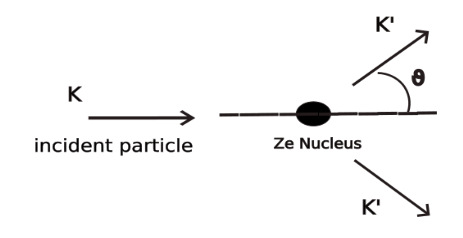
\includegraphics[width = 0.45\textwidth]{ExperimentalSetup/mottFig.png}
\caption{Scheme of the Mott scattering, the polarization is ortogonal to the plane,  $ \vec{n} = \frac{\vec{k} \times \vec{k'}}{|\vec{k} \times \vec{k'}|}$}
\end{figure}

The direction of $\vec{n}$ depends on whether scattering to the left or right is being considered. Let's suppose our initial beam has a polarization $P$, and so we compute the asymmetry $A(\theta)$ of the scattered electrons between left ($N_{L}$) and right ($N_{R}$). $N_{L}$ and right $N_{R}$ will be proportional respectively:


\begin{align*}
N_{L} &= N_{\downarrow}[1 + S(\theta)] + N_{\uparrow}[1 - S(\theta)] \\
N_{R} &= N_{\uparrow}[1 + S(\theta)] + N_{\downarrow}[1 - S(\theta)]  \\
A(\theta) = \frac{N_{L} - N_{R}}{N_{L} + N_{R}} &= \dfrac{N_{\downarrow}(1 + S(\theta)) + N_{\uparrow}(1 - S(\theta)) - N_{\uparrow}(1 + S(\theta)) + N_{\downarrow}(1 - S(\theta))}{N_{L} + N_{R}} = ... = P \cdot S(\theta)
\end{align*}


From the last equation we have a relation which give the beam polarization in terms of $A(\theta)$ (which is what is measured) and the asymmetry function $S(\theta)$ (known also as Sherman function). There are several calculation of the Sherman function, which is well-known for high energy electron scattering.

The total beam polarization is measured by a Moller polarimeter, in the experimental hall, with the beam polarization oriented longitudinally in the experimental hall. The Moller polarimeter can measure the longitudinal polarization of the beam.The other two polarimeters, Compton and Mott, located behind the injector linear accelerator (ILAC), are sensitive to the longitudinal and the trasverse horizontal components of the beam (with an energy around $\SI{3.5}{\mega \electronvolt}$ at this stage). The procedure for the allignment is the following: at the beginning of the beam time the Mott polarimeter is used for different settings of the solenoidal field, with the Wien filter angle equal (nominal) to $\ang{90}$. The aim is to minimize the horizonal polarization component after the rotation performed by the double solenoid, changing the solenoidal magnetic field. Then a second optimization follows, using the Moller polarimeter for different Wien filter angles is performed. With the new Wien filter settings, another measurement is performed with the Mott polarimeter.

\subsection{Moller and Compton polarimeters}


\section{Experimental hall setup.}

\commento{Describing the A1 room, how the spectrometers are operating (+ figures), a picture of the target and the important parameters, like thickness. Also mention the convention to use target with$10 \%$ of the radiation lenght, to avoid double scattering.  Mention that we need the Wobbler magnet to change the hitting position of the beam to prevent the target from melting. Here it's important to mention that the electron are deflected on the vertiacal direction, because of the high beam intensity
Then add a picture of the beam-line.}

Until now we have described how MAMI produce and accelerate the electrons, however we do not presented the structure where the beam is delivered and various experimets are carried out. \\
MAMI has 3 different hall, named with the capital letter A followed with a number, which indicate also the different collaboration that work with the experiments. In A2, as an example, photo-nuclear reactions are studied to investigate the foundamental physics at the scale of nuclear dimensions. The experimental hall where the experiment treated described in this thesis is conducted is the A1 hall. We will describe briefly the main operating detectors that are installed and the details that are interesting for the \transv measurement. \bigskip

\begin{figure}[hbtp]
\centering
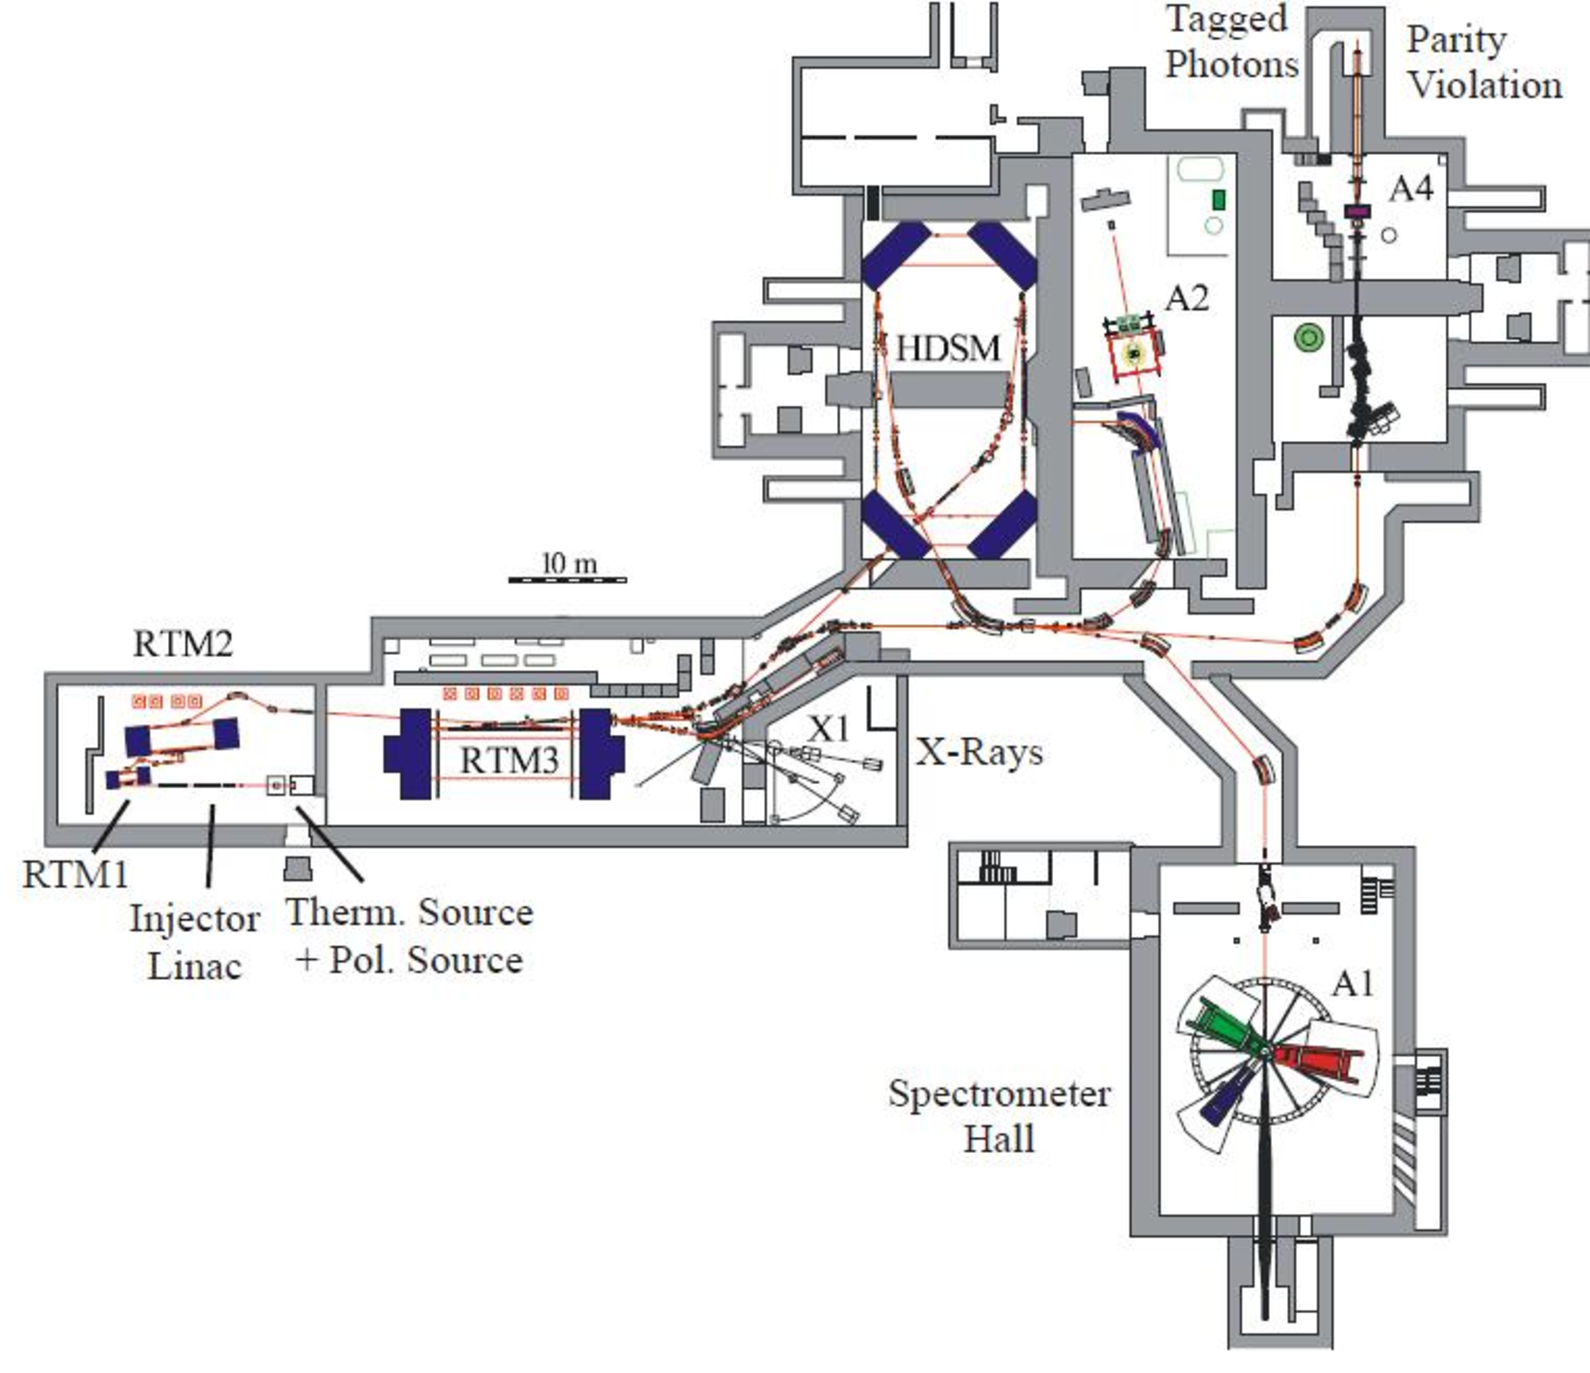
\includegraphics[width = 0.6\textwidth]{ExperimentalSetup/Accelerator.pdf}
\caption{Scheme of the accelerator, with the different experimental hall. Actually the A4 hall is restructured, in fact it will host the future Mesa accelerator.}
\end{figure}

In A1, experiment with fixed target are conducted. The electrons can be delivered with an energy up to $\SI{1.6}{\giga \electronvolt}$, after passing the last acceleration stage (HDSM, in the figure). Because the electron energy of our experiment is $\SI{570}{\mega \electronvolt}$, the beam will pass through the first accelation steps, the linac (linear accelerator) and Race-track system and when the desidered energy is achieved the electrons will be sent to the A1 experimental hall. \medskip

Inside A1 hall three large magnetic spectrometers are placed on a circular railtrack the target chamber. These spectrometers where designed and built in $1993$ to perform high precision measurement of electron scattering in coincidence with other hadron detection, with an high resolution in the determination of the particle momenta $\frac{\delta p}{p} < 10^{-4}$. The spectrometers develop vertically with an height of $\SI{15}{\meter}$, for this reason the scattered electrons and the other particles are deflected with the use of the magnetic field respect to the scattering plane. The following figure shows the path the particle scattered from the target:

\begin{SCfigure}[50][ht]
\centering
\caption{Image of the spectrometers of A1 hall. The spectrometers can be rotated using a system of railtracks that are visible at the bottom of image. The electrons are scattered and then deflected in the vertical direction by the magnetic field (green lines). This picture is taken from behind the target, so we see the beam-dumps. The target is rougly at the center of the image where the two green lines join.}\label{fig:TwoDetectors}
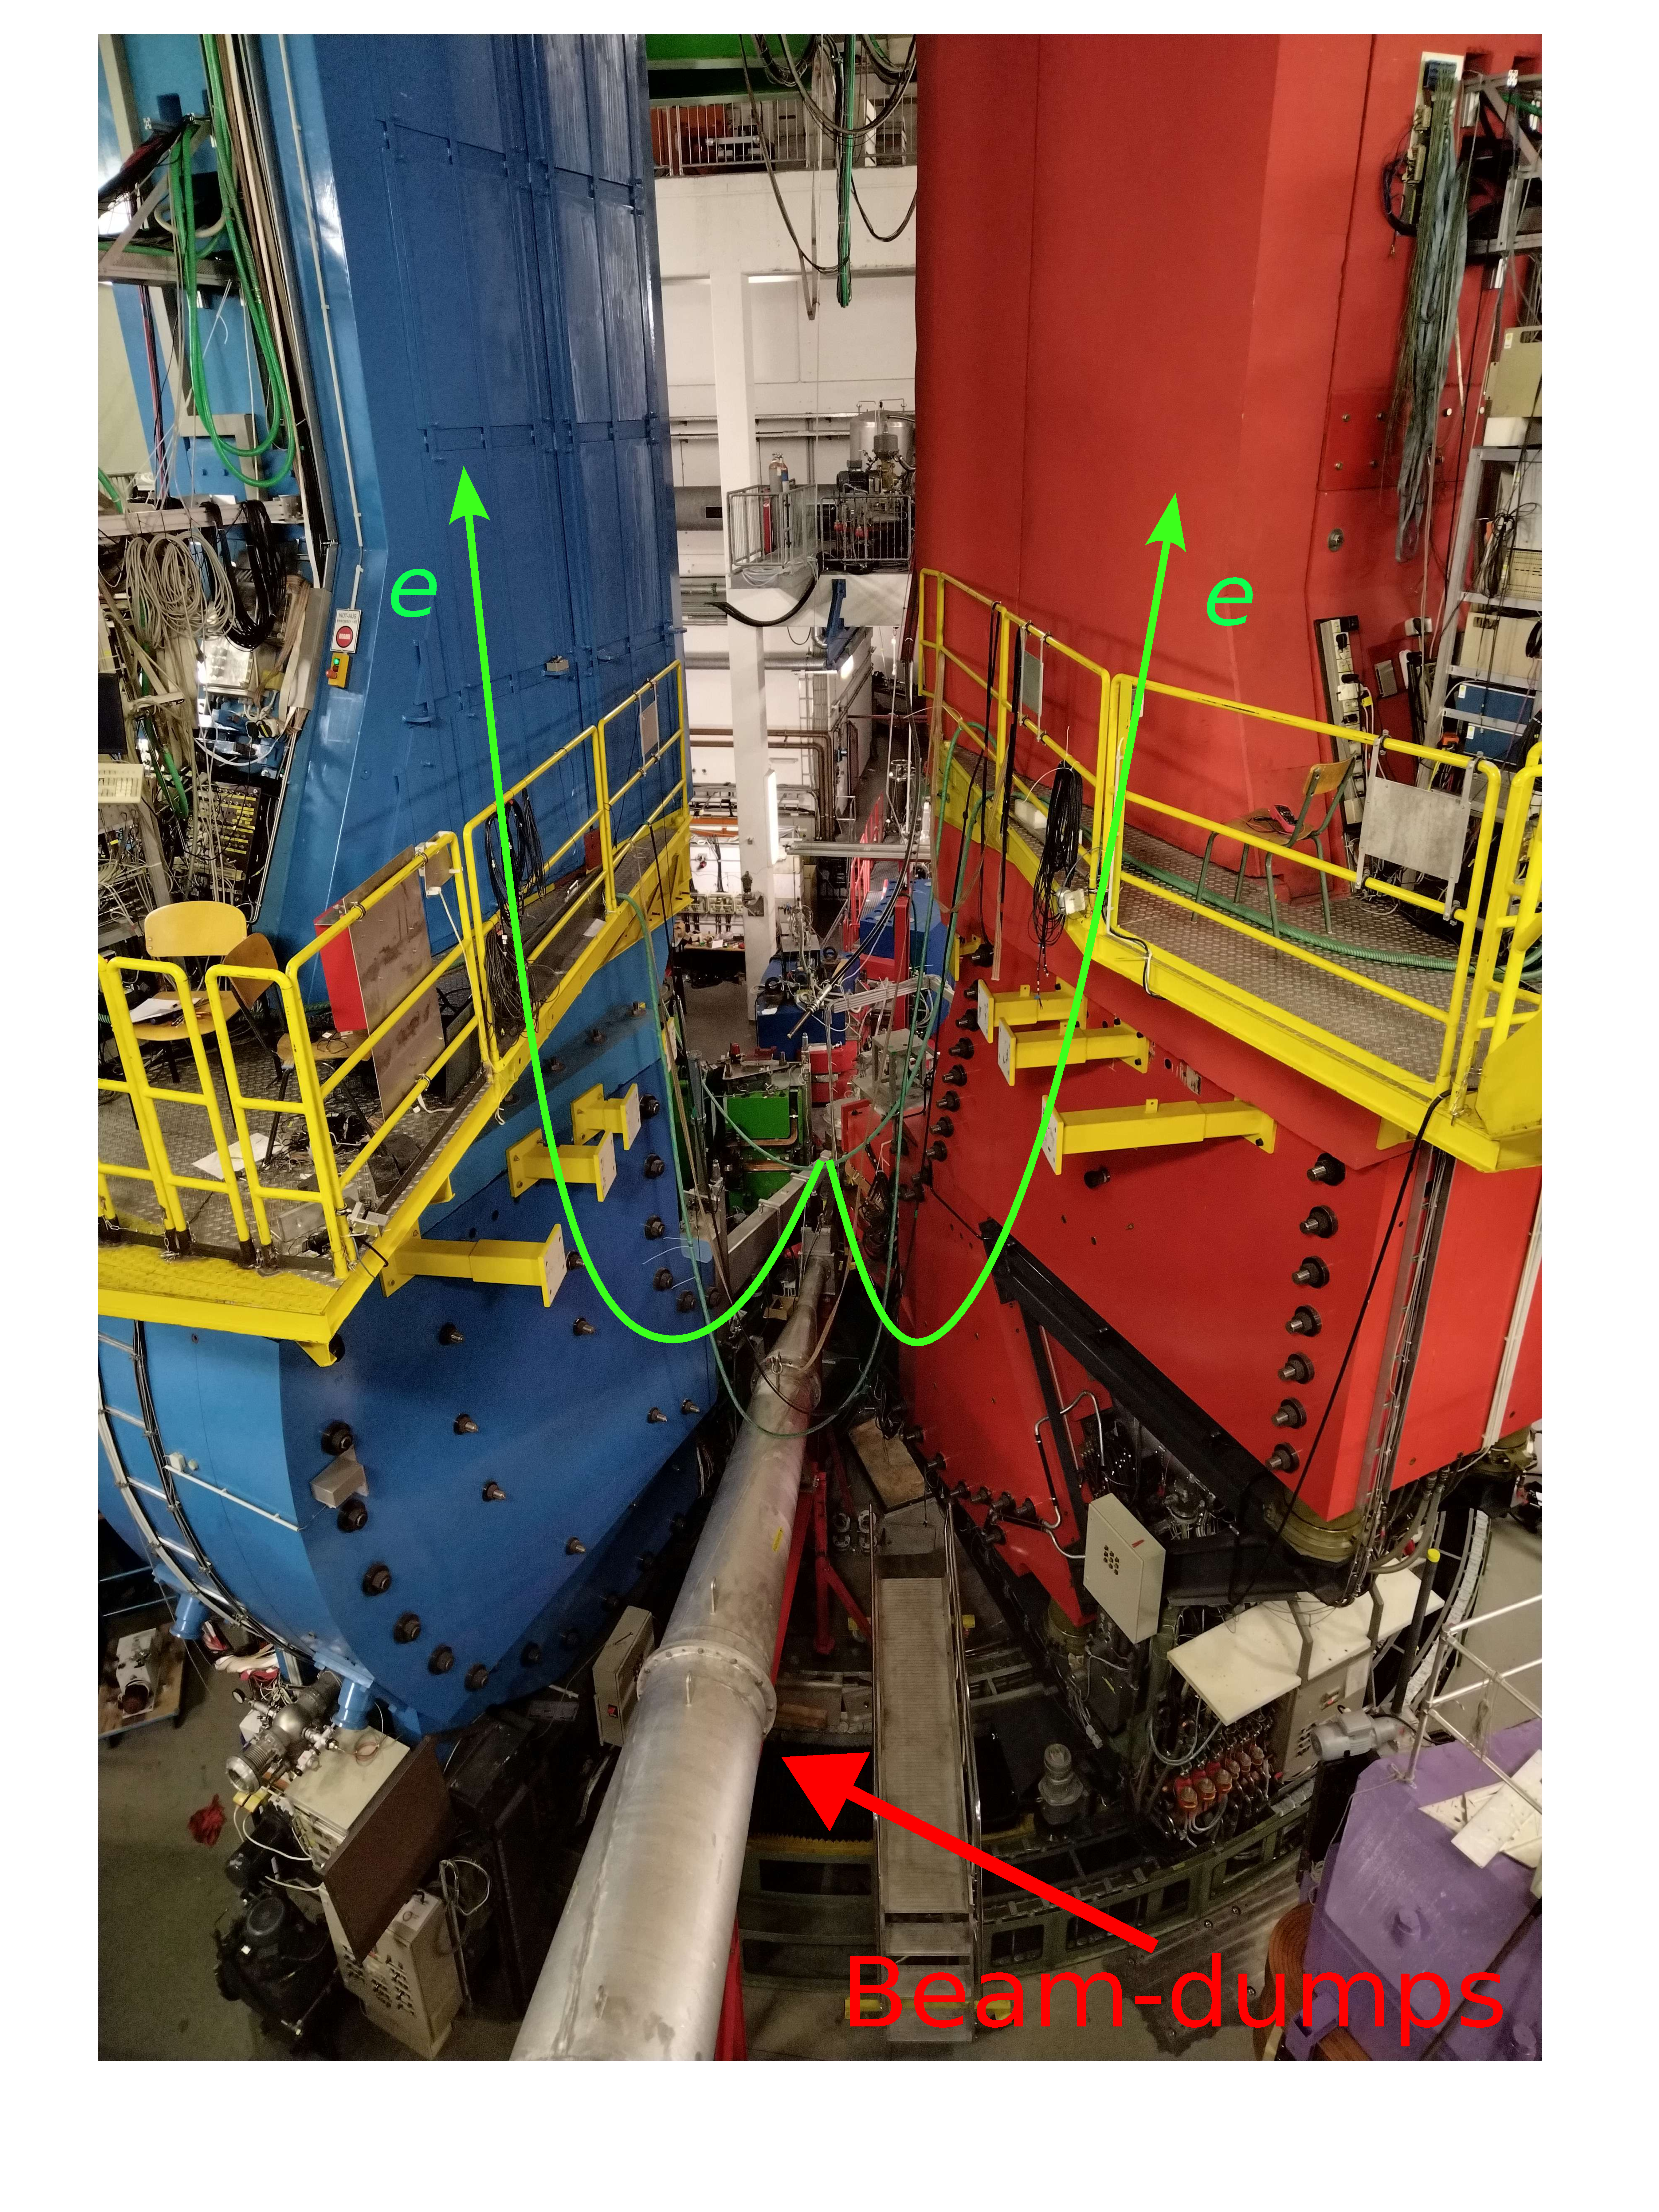
\includegraphics[width = 0.5\textwidth]{ExperimentalSetup/A1_Dietro.pdf}
\end{SCfigure}

The spectrometers used for the \transv are the ones shown in the picture. The are multiple reasons why the particle are deflected on the vertical directon, we summarized them in two points: 
\begin{itemize}
\item reason of space, due to the fact the an horizontal setup would not fit with the dimension of the building in addiction to the fact that this would not allow to rotate the spectrometers by a variety of angles that the vertical orientation does
\item reduce background and noise, in fact the high beam intensity that is possible to reach at MAMI is a source of noise and background event wich can be cut off detecting the particle far from the interaction point. \commento{ultimo punto da verificare!!!}
\end{itemize}      

Once a particle is scattered in the acceptance region of the detectors, the magnetic field deflect the particle that passes through a drift chamber, which occupies the first third in height of the spectrometers. When the particle is at the height of the platform in the figure, it impinge on a layer of plastic scintillator, and after that a Cherenkov detector which measures the particle speed $\vec{v}$. We have a picture of the spectrometers internal, taken during the installation of the two detectors (that will be presented in the next section) \ref{fig:internal}.
\newpage
\begin{SCfigure}[50][ht]
\centering
\caption{Internal of the A spectrometer, the image is taken looking at the detector from the platform in the other image on the left. Normally the walls are closed, this image was taken during the installation of the detector A inside the red spectrometer.}
\includegraphics[width = 0.6\textwidth]{ExperimentalSetup/Detectors/position.pdf}
\label{fig:internal}

\end{SCfigure}

The determination of both the particle speed $\vec{v}$ and momenta (drift chamber) allows to identify the particles. Despite the possibilities offered by the already existing setup, for the beam time of interest none of these components was used directly in the estimation of $A_{n}$. The reason is due to the high intensity of the beam that is used in the experiment, which is far from the optimal operating conditions of the componets, that are suited for rates lower than the ones expected for beam normal single spin measurements. The spectrometers then will de used indirectly for the allignment of scattered electron to

\section{Detectors and beam monitors}

\subsection{Detectors A and B}
\commento{Describe the two detectors we placed inside the spectrometers, the $Q^{2}$ for our mesurement. The way the counts are collected, so the expected signal for the Čerenkov detector. Explain also how we will use the old detectors of the two spektrometers to align the elastic scattering plane to our detectors.
\begin{itemize}
\item explain the two detector, the type of cristal used. 
\item how the pmt are coupled to the cristal, the number of dynodes of the pmt, the power supply.
\item add an picture/scheme of the pmt.
\item explain why a diffusor is not needed.
\item what kind of optical coupling is used?
\item dimensions of the two detectors.
\end{itemize}
}


In this section we will describe the electronics and the detectors used to measure the \transv .
For this experiment we are going to measure the \transv at to different agles. The electrons detection is 
made via two thin blocks of fused-silica that are coupled to pmts. When a scattered electron hit the fused-silica (refractive index $n = 1.45$) Cherenkov light is emitted. The emitted cherenkov light can interact with the electrons of the material, which, in turn, can hits the PMT dyode. This sequence of event triggers the pmt and produce an output signal.

In the experiment, we will measure the \transv at two angles of scattering, so two detectors are installed and read-out indipendently. The two detector are made by 3 PMTs and 8 PMTs coupled with two blocks of fused-silica, a scheme of the detector is shown below:

\begin{figure}[hbtp]
\centering
\subfloat[][\emph{Detector B scheme.}]{
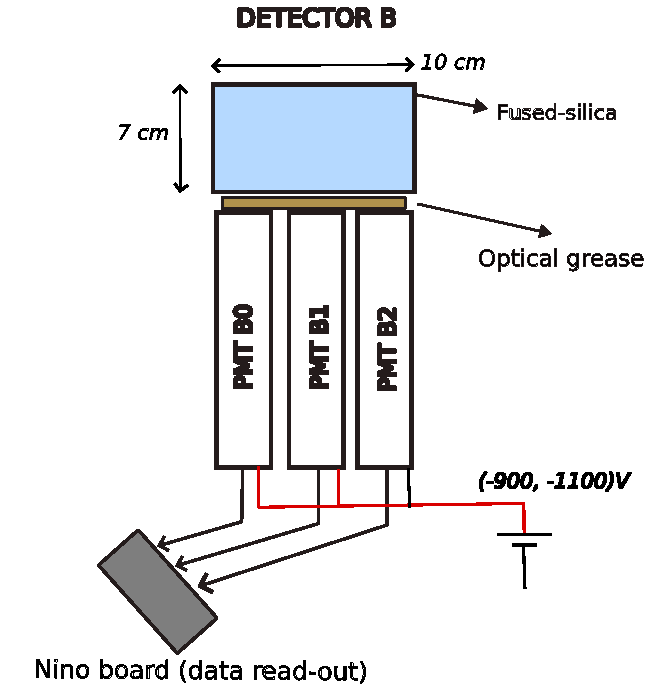
\includegraphics[width = 0.40\textwidth ]{ExperimentalSetup/Detectors/DetectorB.pdf}}
\subfloat[][\emph{Detector A scheme.}]{
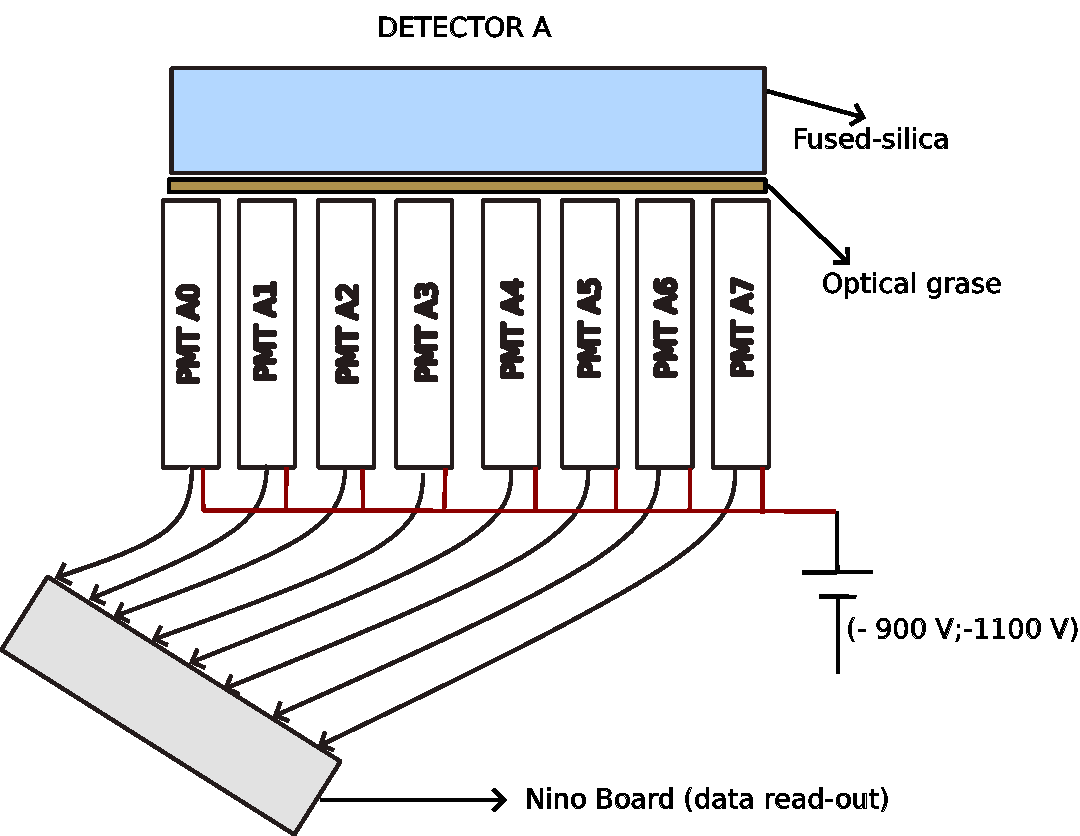
\includegraphics[width = 0.55\textwidth ]{ExperimentalSetup/Detectors/detectorA.pdf}}
\end{figure}


These  two detectors are placed inside the spektrometers presented in \commento{aggiungere referenza}, between the top of the drift-chamber, which occupies the first third in height of the spectrometer, and just below a panel of scintillator. During the beam time the drift chamber of the spektrometers is turn off, and also the pmts coupled to the spektrometer scintillators are not powered.\\
As we mention above, the scattered electron are deflected in the vertical direction by the magnetic field of the spektrometer. 
At this moment, it is important to mention the differencies between the new and the old electronic setup. In the old electronic setup the output signal of the pmts was integrated during the time interval of each sub-event, and therefore the single scattered electron could not be counted. The advantage of this method is that the electronics is more simple, in fact there in no need to develop a fast counter, unlike the new setup, where the new electronic take into account of every pulses. However, this old method is effected by a baseline noise and it's not good for the future experiments with lead target, where the expected rates are lower than the rates on carbon.
With the new electronics, all the single electron are counted, and this will allow the future measurements with lead, improving the accuracy. 

\begin{figure}[hbtp]
\centering
\subfloat[][\emph{Detector B}]
	{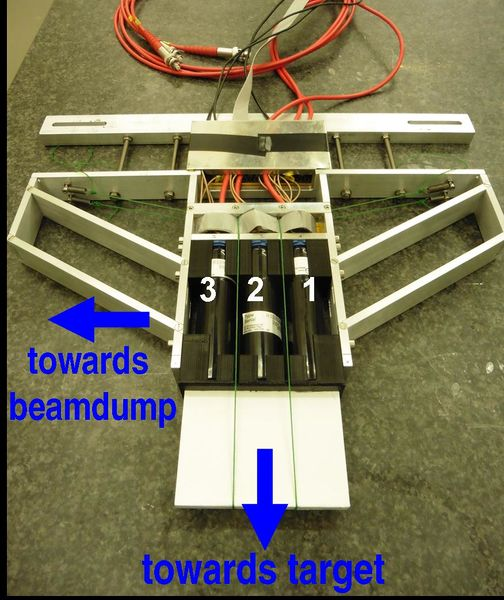
\includegraphics[width = 0.35\textwidth]{figures/504px-Blackfalcon.jpg}} \quad
\subfloat[][\emph{Detector A}]
	{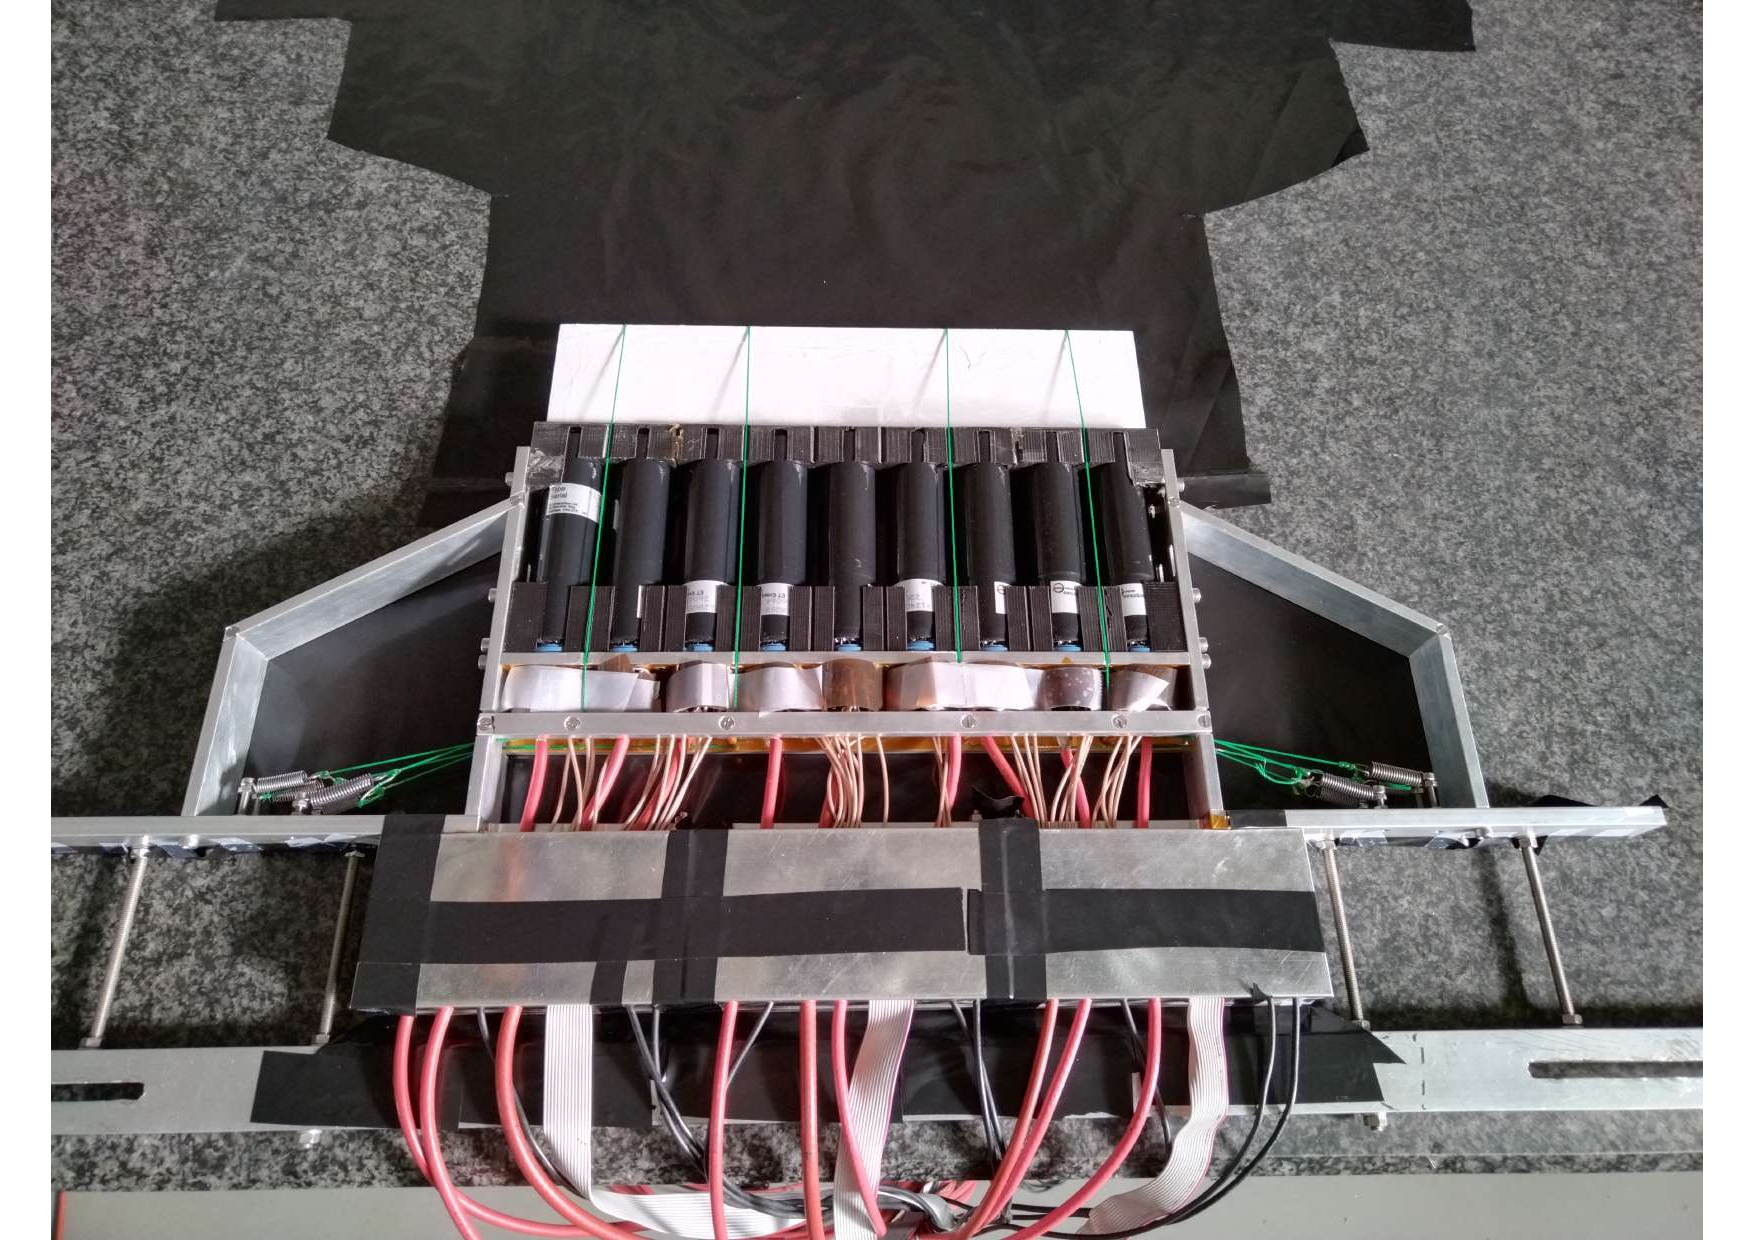
\includegraphics[width = 0.45\textwidth]{figures/IMG_20221110_122246.jpg}} \quad
	\label{fig:Detectors}
\caption{Picture of the two detector taken in the clean room. The white blocks are the fused silica that produces the Cherenkov light, the cylinders below are the PMTs.}
\end{figure}

Here we report the characteristic of the two detector that are relevant for the data analysis: 

\begin{itemize}
\item detector B size (lenght, hight, depht): $\SI{7}{\centi \meter} \times \SI{10}{\centi \meter} \times \SI{1}{\centi \meter}$
\item detector A size (lenght, hight, depht): $\SI{7}{\centi \meter} \times \SI{30}{\centi \meter} \times \SI{1}{\centi \meter}$
\item Number of dynodes: \commento{inserire il numero di dynodes, magari un accenno all'amplificazione}.
\item The Power voltage for the pmt in negative, in the range of ($\SI{-900}{\volt}$, $\SI{-1100}{\volt}$)
\item refraction index $n$ of the fused-silica is $1.45$.
\end{itemize}


\subsection{Beam monitors.}
\commento{Explain how the monitors for the beam parameters work. (this section could be long, however the way these parameters are measured is particular, so it's important to explain everything properly).}

In MAMI, several monitors are placed along the beam line in order to to check beam quality and measure parameters such as current intensity, energy and relative position of the beam. This section summarize an explanation of the operating principles of the monitors installed at MAMI. The explanation will be partial, some details will be given in the appendix, however for a complete discussion please refer to the following paper ( \cite{M_Dehn}).

The monitors avaible at MAMI are quite specific for the standard of the particle accelerators. Resonant cavities are used to measure the various quantities, with the underlying physical principle that the passage of charged particles through these cavities can excitate some electromagnetic resonant modes\footnote{TM mode, where the magnetic field is completely trasverse respect to particle momenta} which can be detected and analyzed by an analogic circuit to measure the beam parameters.
Before going into the details, is necessary to define some quantities that will be used later in the explanation. We define $r_{s}$, the Shunt-impendence as :

\begin{equation}
r_{s} = \frac{|V_{\|}|^{2}}{P}
\end{equation}

$P$ is the power absorbed by the cavity when a particle excites one of the resonant mode, instead $V_{\|}$ in defined as the effective voltage surpassed by a charged particle along a straight line, which can be computed as:

\begin{align*}
V_{\|} = \frac{1}{q}  \int_{s_{0}}^{s^{1}} \vec{E}_{s} \vec{e_{s}} \,ds
\end{align*}

The Shunt impedence is a measure of the interaction strenght between a cavity and a charged particle, and can be espressed also in another way, introducing the $Q$ value of the cavity, $W$ the maximum energy stored and $f_{r}$ the frequency of resonance:

\begin{align*}
r_{s} = \dfrac{|V_{\|}|^{2} Q}{2 \pi f_{r} W}
\end{align*}

When the beam travel through the cavity, the particles release enery that excites the oscillascion mode. The power $P_{HF}$ extracted from the beam is related to the beam current: 

\begin{align*}
P = \iota^{2} r_{s}
\end{align*}

An antenna is used to decouple part of the energy from the cavity and send it to a circuit which produces an analog output signal. Indicating with $\kappa$ the coupling costant of the antenna, the previous relation need to be modified introducing a new factor $ \frac{\kappa}{(1 + \kappa)^2}$. In a Cylindrical resonator, the same type installed at MAMI, the resonance frequency of the different oscillascion modes is expressed by the formula 

\begin{align*}
f_{m,n,p} = \frac{c}{2\pi \sqrt{\epsilon_{r} \mu_{r}}} \sqrt{(\frac{x_{m,n}}{R})^{2} + (\frac{p \pi}{L})^{2}}
\end{align*}

The costant in the formula are:

\begin{itemize}
\item $c$ is the light speed.
\item $\epsilon_{r}, \mu_{r}$ are the magnetic and dielectric costant of the material.
\item $x_{m,n}$ it the n-th zero of the m-th Bessel function.
\item $R$ and $L$ are the radius of the cylindrical cavity and his lenght.
\item \commento{$p$ I dont' know yet.}
\end{itemize}

This formula can be obtained solving the Maxwell equations with cylindrical boundary condition, the eigenvalues are the given by the formula above. \\
If the frequency of the Beam bunch is equal to the resonant frequency $f_{m,n,p}$ of the cavity, a TM mode is excited. At MAMI high quality monitors are installed, quantitatively all the monitors have a $Q \simeq 10000$, that means that $\frac{\nu}{\delta \nu} \simeq 10000$. This means that the frequency of the beam buch must be very close to the frequency of the resonant cavity. At MAMI the frequency used for all the resonators is $\SI{2.449532}{\giga \hertz}$ or a multiple of it. The beam bunch frequency is the same, and it's controlled by the MAMI-master oscillation signal, that is the reference signal for all the MAMI monitors.

\begin{figure}[hbtp]
\centering
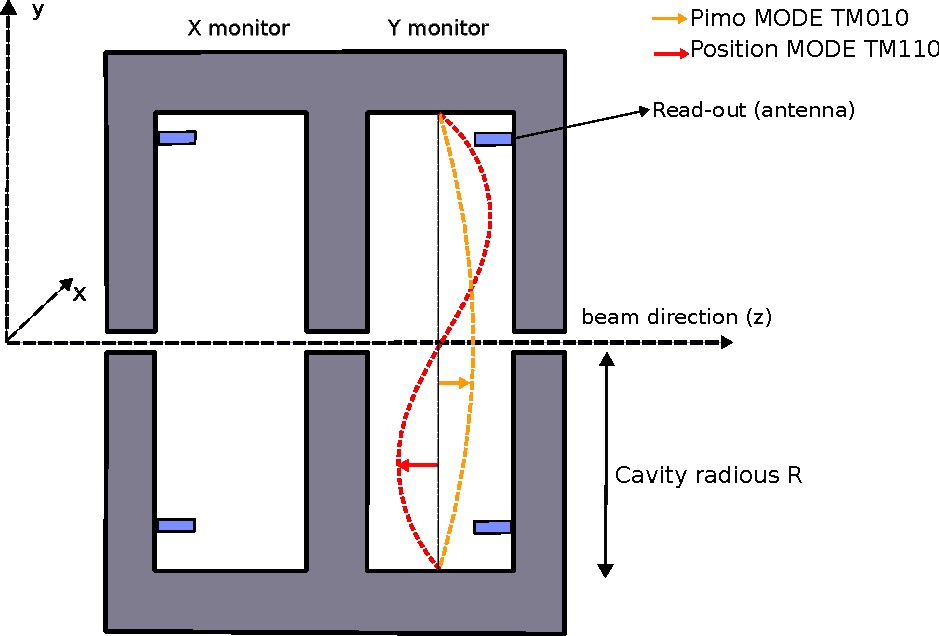
\includegraphics[width = 0.6 \textwidth]{ExperimentalSetup/Monitors.pdf}
\caption{Scheme of the Cylindrical cavities installed at MAMI. In red we have the $TM_{110}$ mode, used to measure the position of the beam, in yellow the $TM_{010}$ mode, to measure the intensity of the beam.}
\end{figure}

Depending on the $TM$ mode excited, we have a different signal in the cavity, so a different signal collected by the antenna. The relevant quantity that is detected is the power $P_{HF}$ absorbed by the antenna. For the $TM_{010}$ mode, the power is 

\begin{equation}
P_{HF} = i^{2} r_{010} \frac{\kappa}{(1 + \kappa)^{2}}
\end{equation}

The power absorbed by the antenna is directly dependent on the beam current. Because the rage values are typically in the range of $\SI{}{\pico \watt}$ to $\SI{}{\milli \watt }$, the signal is processed in close proximity of the installed monitors. In the signal process, the input signal of the antenna in coupled to the master-oscillascion signal, so the output signal is given by the formula:

\begin{equation}
U = \sqrt{P_{HF}} \cos(\phi - \phi_{LO})
\end{equation}

the phase $\phi$ is the phase of the resonant mode or the phase of the beam bunch, while the phase $\phi_{LO}$ is the phase respect to the master-oscillation signal, and can be adjusted by a phase shifter of the circuit. The output voltage signal can be read out with the oscilloscope or digitalized and saved with other devices. To measure the beam intensity is important to minimize $\phi - \phi_{LO}$, to maximixe the signal amplitude, and then the output signal is ready to be analyzed. \\
The measurement of the $x,y$ position follows in principle the same procedure. In this case the $TM_{110}$ is acquired. The reason is clear, because it's possible to calculate that for this mode the $r_{shunt}$ is proportional to the beam position on the $x,y$ plane. So The power absorbed by the antenna can be written:

\begin{equation}
P_{HF} = i^{2} r_{110} \frac{\kappa}{(1 + \kappa)^{2}} K x^{2}
\end{equation} 
 
with the output signal prortional to the square root of the absorbed power, we end with:

\begin{equation}
x,y = \sqrt(P_{HF}) = costant \cdot \frac{U}{i}  
\end{equation} 

With this is clear how it's possible to measure all the important quantity related to the beam that will be used for the analysis.

\subsection{Beam stabilization.}

\section{Electronics}
\commento{Short introduction about the old electronics setup and why a new versions is needed, then describe all the electronics used for our experiment:
\begin{itemize}
\item Nino board for collecting the data from the pmts
\item VFCs for collecting the data from X21,X25,Y21,Y25,ENMO,I21,I13
\item master board for collecting the monitors data/controlling the source/wobbler magnets.
\item small boxes for switching from new electronic read-out to the old electronics read-out (spectrometers DAQ)
\end{itemize}}


\subsection{VFCs}

Some parameters which describe the beam are needed in order to take into account possible effect in the measure of the Trasverse asymmetry. The relevant data are the position in the $(x,y)$ plane, the incident angles on the target, the current and energy of the beam. All this values are collected using the already existing monitors. \\
To collect the data from the monitors, single and multichannel, synchronous voltage-to-frequency converters (AD7742) are used. This devices contain an analog modulator that is able to convert the input voltage into an output pulse train, whose frequency is proportional to the input voltage. 

\begin{wrapfloat}{figure}{I}{0pt}
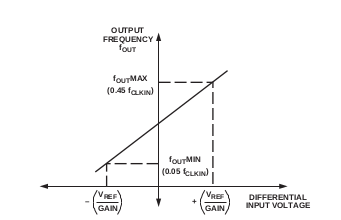
\includegraphics[width=0.5\textwidth]{ExperimentalSetup/Vfc.png}
\caption{Frequency versus Voltage}
\end{wrapfloat}

The VFCs are powerd with an external tension of $\SI{5}{\volt}$, and a differential voltage input in the range ($-V_{ref}$, $V_{ref}$) is also applied. An external clock signal, that is indicated with "CLKIN" is provived as a reference signal for the oscillator frequency.
The analog input signal is sampled with by a switched capacitor, with a rate that is controlled by clock  that can be supplied externally, in our case we used a $\SI{6}{\mega \hertz}$. A scheme of the electronic circuit is drawn here (\textit{aggiungere figura}), the output of the Comparator  is a fixed width pulse (the pulse is initiated by the edge of the clock signal) with a frequency that goes from $0.5 \% \cdot f_{CLKIN}$ to $0.45 \% \cdot f_{CLKIN}$ \cite{VfcDatasheet}, where the first correspond to $\SI{0.0}{ \volt}$ in input and the second to $V_{ref}$. Neglecting possible systematic errors, the relation the output frequency and the input voltage is the following:

\begin{equation}
V_{in} = \frac{V_{ref}}{40 \% \cdot f_{CLKIN}} (f_{out} - 5\% f_{CLKIN})
\end{equation}

We control the $f_{CLKIN}$ with the period of the clock. The data are acquired counting the number of pulses that come from the comparator, so we can substitute to $f$ the number of pulses (the two quantities are proportional), and we end with:

\begin{equation} \label{eq:Vfc}
V_{in} =  V_{ref}[2 \cdot \dfrac{N_{pulses} - 5 \% N_{CLKN}}{40 \% N_{CLKN}} - 1]
\end{equation}

\subsection{Nino board} \label{NINO}

The NINO board is our data acquisition system for the pmt counts. It is made by $32$ analog input channels and it'is power with $\pm \SI{5}{\volt}$. Each channel has an attenuator, and the signal pass through that before going to the Comparator, which compare the signal to the threshold. The Output signal is a Low-voltage differential signaling (LVDS). Each comparator can handle eight channel and for each of them it is possible to define a global threshold. With the current settings of NINO board, it is possible to change the threshold of each channel acting on another value, the attenuation, which decreases the value of the global threshold of each single channel. All the value that can be modified are 12 bit numbers, so a setting interval of $(0. ; 4095)$.

\begin{figure}[hbtp]
\centering
%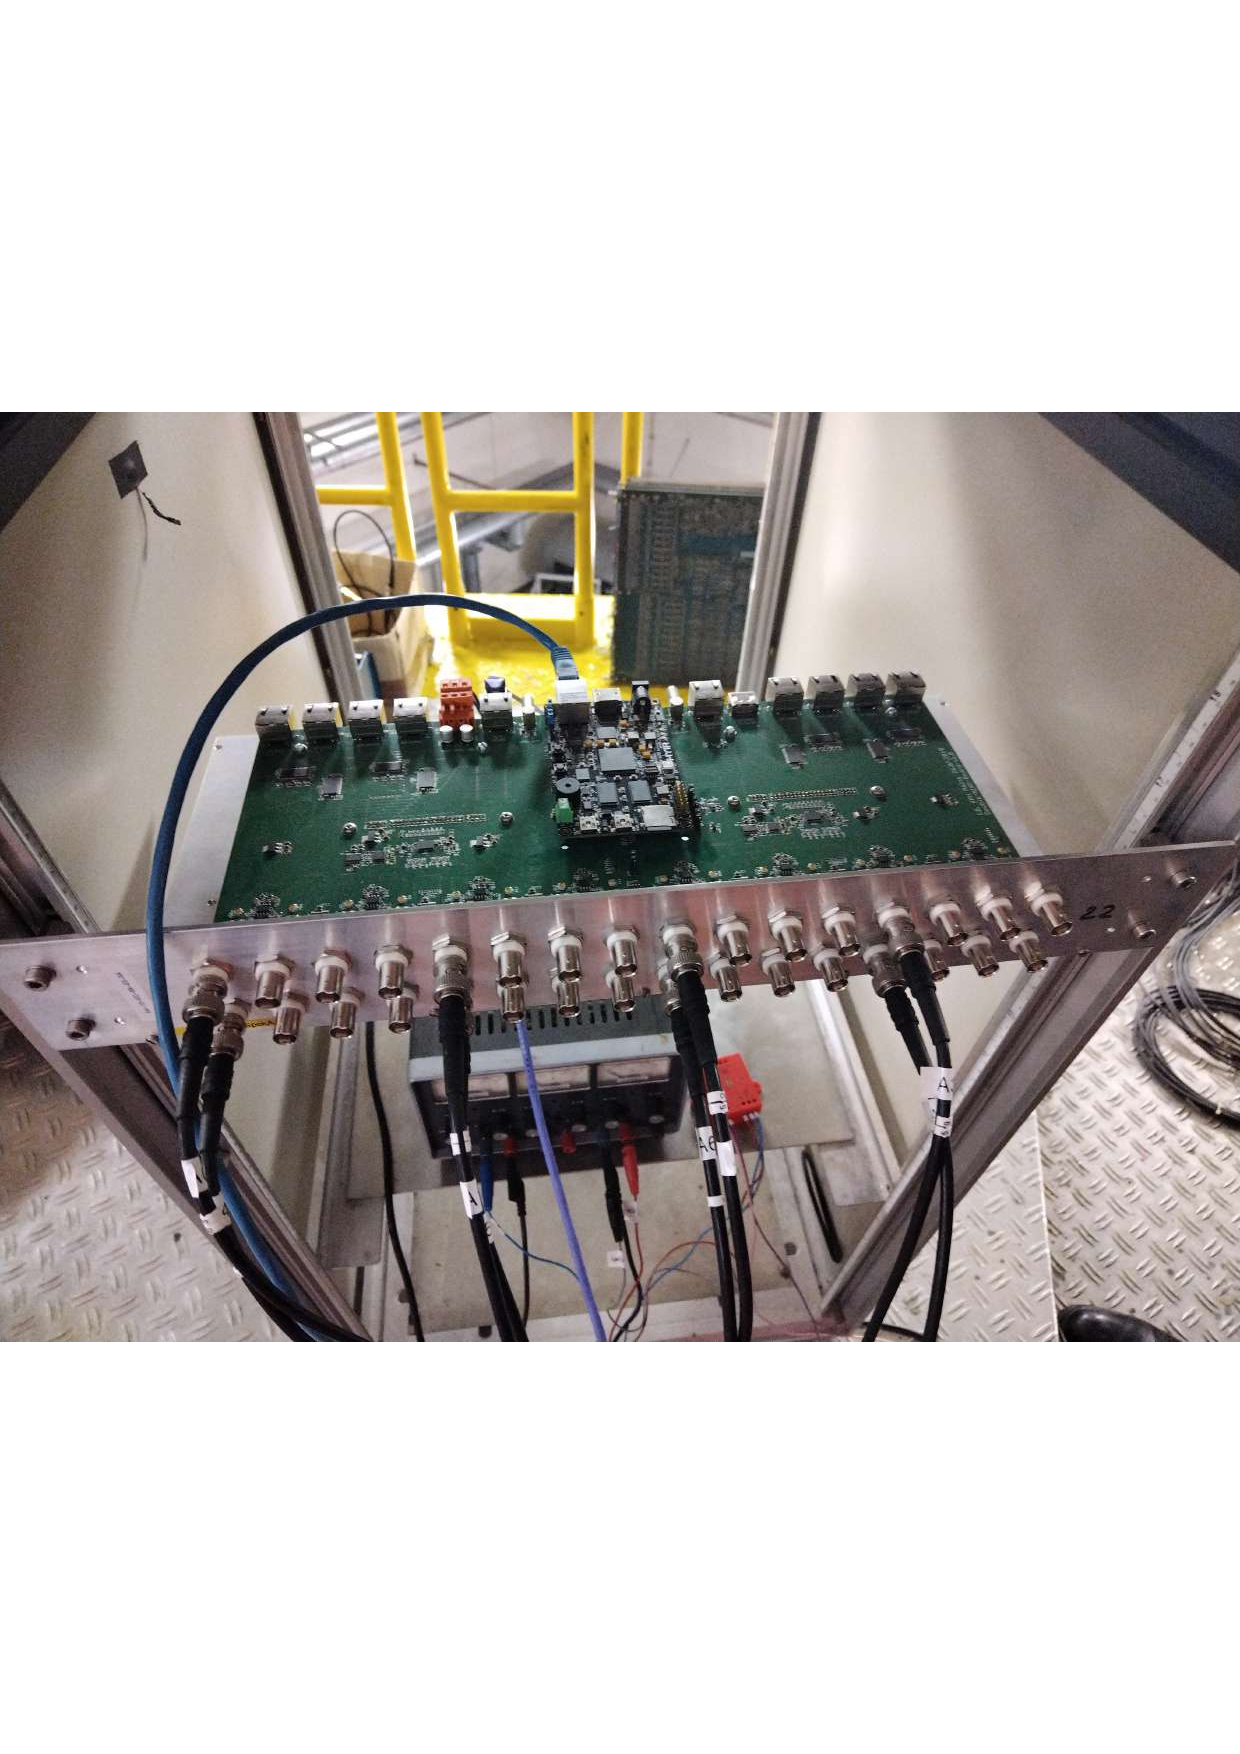
\includegraphics[scale= 0.4]{figures/NINO.pdf}
\caption{Nino Board}
\label{fig:NinoBoard}
\end{figure}

Two Nino board are used in the experiment, one for detector A and one for detector B. In principle it is possible to use only 8 and 3 of the 32 channels the are ready to use, considering we have only 3 and 8 pmts to read out. However it is useful to split the analog output signal by the pmts and send it to 4 different channels. So, working with the attenuation value, we can define 4 different threshold values for each pmt. This is something that can improve the noise management. This will be implemented for the future experiments, nevertheless this was not done during our data collection.
The way we selected the threshold is explained in the following chapter (Analysis).

\subsection{Master Board}